\documentclass[UTF8]{article}

\usepackage{amsmath}%数学符号
\usepackage{hyperref}
\usepackage{xeCJK}
\usepackage{pgfplots}
\usepgfplotslibrary{dateplot}
\usepackage{makecell}
% \usepackage{multirow}


\newcommand{\ud}{\mathrm{d}}%定义微分符号为竖直罗马体


\title{Yelp Review Prediction}
\author{Yifan Li}

\begin{document}

\maketitle

\section{Introduction}

This project aims to:

\begin{enumerate}
\item find a explainable model to predict the score consumers will give (from 1 star to 5 stars) with their reviews.
\item find patterns of positive reviews (4-5 stars) and negative reviews (1-2 stars).
\item classify words into positive and negative.
\end{enumerate}

Data I used is download from \href{https://www.yelp.com/dataset}{Yelp website}. It contains about 1.5 million reviews with several columns. Only the \textit{review} and \textit{score} columns are used in this project.

The main idea of the model is to classify positive and negative words using the frequency ratios that each word appears in positive and negative reviews. And use the frequency of different types of words to classify positive and negative comments.

\section{Method}

\subsection{Clean Data}

\paragraph{Abbreviation and Special Symbols}

First, abbreviation and special symbols are modified. After the inspection, there exists eight situations.

\begin{table}[!htb]
    \begin{tabular}{|l|c|c|c|c|c|c|c|c|}
    \hline
    Origin & n't & 's & 've  & 'd    & 'm & lve    & cannot  & \textbackslash{}n              \\ \hline
    Now    & not & is & have & would & am & I have & can not & \textless{}Space\textgreater{} \\ \hline
    \end{tabular}
\end{table}

\newpage

Here are some examples:

\begin{table}[!htb]
    \begin{tabular}{|l|l|}
    \hline
    Origin                                                       & Now                      \\ \hline
    Long story short.\textbackslash{}n\textbackslash{}nBunch ... & Long story short. Bunch  \\ \hline
    We didn’t catch her ...                                      & We did not catch her ... \\ \hline
    It’s super clean ...                                         & It is super clean ...    \\ \hline
    \end{tabular}
\end{table}



\paragraph{Non-English} 

Non-English reviews are removed. Here are some examples:

\begin{table}[!htb]
    \begin{tabular}{|l|}
    \hline
    2ème arrêt au Barbù et nous avons vécu une,...    \\ \hline
    Corriente, sucio, y mal servicio. El cocinero,... \\ \hline
    アリゾナ 最後に 良い旅の想い出の締めくくり,...                        \\ \hline
    家から最寄りで食べに行けるベトナム料理 ...                           \\ \hline
    \end{tabular}
\end{table}

They only account for one percent of the total reviews. So I directly delete them.

\paragraph{Negative Sentence} 

The last and most important part is to deal with negative sentence. For examples, \textit{brightest} is obvious a positive word. However, when it occurs in a sentence like "there were not the brightest person", it actually functions as a negative word. If we remain considering it as a positive one, it will ruins our prediction. For instance, words \textit{well} and \textit{return} which exists in the  review "the staff were obviously not well managed, I will never return to this location." are both positive while this review brings no obvious negative word. Without special adjustment, this review will usually be taken as positive review in regression and given a high score. However, it is actually a one star review.

My idea is first finding words which makes a sentence as negative sentence. After checking several sentences, four words are found. They are \textit{no, not, never, lack}. Sentences with these four words are usually negative sentence. I call them inverters. Then, for each negative sentence (sentences including inverters), I add a \textit{not} in front of each word between inverters and the following punctuation. Here are some examples:

\begin{table}[]
    \begin{tabular}{|l|l|}
    \hline
    Origin & \makecell{the staff were obviously not well managed, I will never return to this \\location}               
    \\ \hline
    Now    & \makecell{the staff were obviously not notwell notmanaged, I will never notreturn \\notto notthis notlocation }\\ 
    \hline
    Origin & Seriously can not stand this McDonald is. They never get my orderright.  \\ 
    \hline
    Now    & \makecell{Seriously can not notstand notthis notMcDonald notis. They never \\notget notmy notordernotright.}   \\ 
    \hline
    \end{tabular}
\end{table}

\newpage

Now, with \textit{good} and \textit{notgood}, we can determine whether it is in a positive sentence or negative sentence.

After doing all transformation, I delete all punctuation. It will lose some information. \textit{!} or \textit{?} may bring some special information. But I have no idea to analysis them. And I believe words is enough.

Due to the limitation of my computer, I randomly choose 100,000 reviews from total 1.5 million reviews to do further analysis.

\subsection{Determine Positive and Negative Words}

The most intuitive method to determine positive words is to rank words with their frequency of appearing in positive reviews (4 or 5 stars reviews). However, there is a big problem here. Some meaningless words appears significantly more frequent than other words. For example, the word \textit{is} appears 6467 times among all 10,454 1 star reviews while the word \textit{disrespectful} appears only 42 times. If we merely consider the frequency or equivalent probability, \textit{is} will be taken as negative and \textit{disrespectful} won't seem to be so negative. However, we know the opposite is true.

To avoid this kind of misclassification, probability ratio is used instead. I create five new variables named as Score1 to Score5. For example, the definition of Score1 for a word is:

\[
\text{Score1[word]} = \frac{P(\text{this word is included in reviews with 1-star})}{P(\text{this word is included in reviews with stars other than 1})}    
\]

Definitions of Score2 to Score5 are similar, which just replace 1-star with 2-5 stars. Here are some examples to show the power of these five new Score variables.


\begin{table}[ht]
\centering % used for centering table
\begin{tabular}{l l r r r r r r} % centered columns (4 columns)
	\hline %inserts double horizontal lines
	Word   &Variable  & 1-star & 2-star & 3-star & 4-star & 5-star  \\ [0.5ex] % inserts table
	%heading
	\hline % inserts single horizontal line
    \textbf{worst}         & frequence   & 1310   & 332     & 150     & 80      & 40      \\ 
    \cline{2-7} 
    & probability & 1e-3   & 4e-4    & 1e-4    & 3e-5    & 2e-5    \\ 
    \cline{2-7} 
    & Score       & 18.3   & 1.9     & 0.5     & 0.107   & 0.038   \\ 
    \hline
    \textbf{notregret} & frequence   & 7      & 5       & 10      & 70      & 177     \\ 
    \cline{2-7} 
    & probability & 8e-6   & 5e-6    & 8e-6    & 3e-5    & 8e-5    \\ 
    \cline{2-7} 
    & Score       & 0.225  & 0.172   & 0.227   & 0.865   & 3.420   \\ 
    \hline
	\hline
    \textbf{and}            & frequence   & 8943   & 8623    & 12542   & 25459   & 31314   \\ 
    \cline{2-7} 
    & probability & 0.0097 & 0.0093  & 0.0095  & 0.0111  & 0.0134  \\ 
    \cline{2-7} 
    & Score       & 0.964  & 0.999   & 0.992   & 1.020   & 1.000   \\ 
    \hline
\end{tabular}
\caption{Score of Words}
\label{table:score}
\end{table}

From Table \ref{table:score}, we can see that although word \textit{and} appears frequently, its distribution in reviews with stars is approximate uniform. And its Score1 to Score5 are closed to 1. However, for negative word \textit{worst}, its Score1 is obviously larger than other scores. For positive word \textit{notregret}, its Score1 is obviously larger than other scores. (remember \textit{not} in front of \textit{regret} indicates that it is a negative sentence like "you will never regret". So that \textit{notregret} is positive)

Here are two word cloud plot of words with high Score5 and Score1.

\begin{figure}[htbp]
    \centering
    \begin{minipage}[t]{0.5\textwidth}
    \caption{Positive}
    \centering
    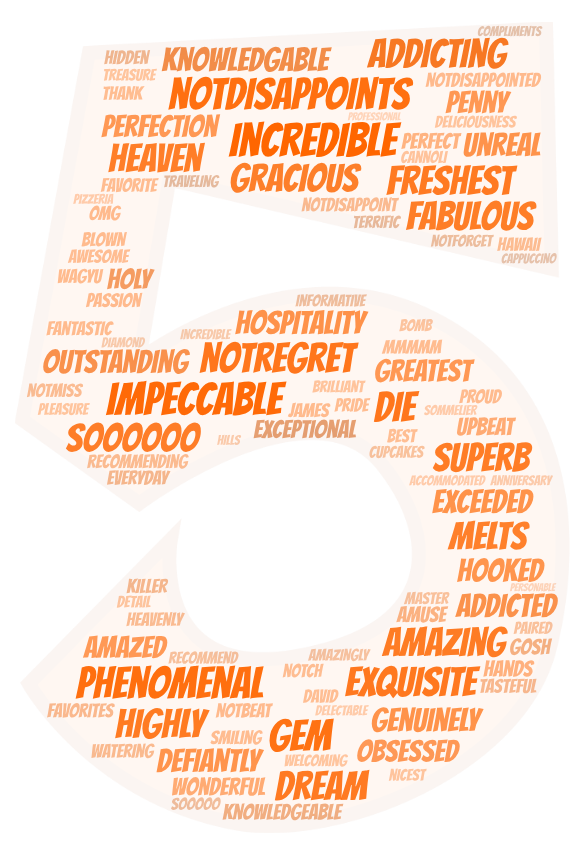
\includegraphics[width=4.8cm,height=7.75cm]{../image/5.png}
    
    \end{minipage}
    \begin{minipage}[t]{0.48\textwidth}
    \caption{Negative}
    \centering
    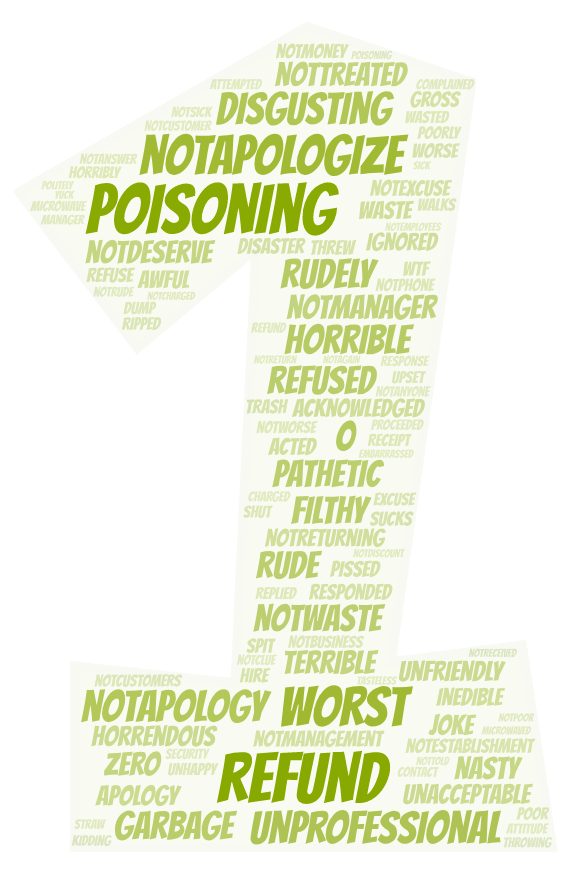
\includegraphics[width=4.8cm,height=7.75cm]{../image/1.png}
    
    \end{minipage}
\end{figure}

Here are some interesting findings. \textit{die} is positive and \textit{refund} is negative. I check some reviews which include these words. 


\begin{enumerate}
\item i was told that our order would be \textbf{refunded}. as of the following tuesday it had not.
\item they refused to \textbf{refund} our money
\item the cake was so beautiful and absolutely to \textbf{die} for!!!!
\end{enumerate}

When customers consider refund, it is not a good signal.

\subsection{Determine Positive and Negative Reviews}

After giving scores to words, now I need to give scores to reviews. Another five  new variables S1 to S5 are created. For example, the definition of S1 of a review is:

\[
\text{S1[review]}=\text{\# of words with high Score1 in this review.}    
\]

After ranking by Score1, the first 1000 words are taken as "words with high Score1".

Definition of S2 to S5 is similar to S1. Now we can use these variables to do prediction.


\section{LSTM model}

Finally I fit a LSTM(Long Short-Term Memory) network of star$\sim$ S1+S2+S3+S4+S5. Details of my model could be found in "LSTM.ipynb" file. After cross validation, the total MSE is 0.63310782. Compared with least square lineal model, its MSE is about 1.1. It means LSTM network is a great improvement of lineal model. 

Actually when I use the whole data set and take 80\% as train data and rest 20\% as test data, MSE of my model once reached 0.281. But due to the limitation of my computer, I can't do cross validation on the whole data. So I don't know whether there is any bias in splitting data.

\section{Conclusion}

\begin{enumerate}
\item Score1 to Score5 are powerful variables to determine a word positive or negative.
\item Although LSTM network is not interpretable, variables used in this model are interpretable.
\item My model is simple and basic but it still achieves good results. It means actually variable selection is more important than model selection in this situation.
\item There is no special reason to choose LSTM other than neural net model. So in the future, I could try other neural net model and do grid search over various model parameters to improve predictions.
\item Words with high Score1 and low Score1 have the same contribution on S1. Maybe I should try to allow different weights on them.
\item I find that negative reviews usually are longer than positive reviews. The length of reviews as a new variable may be helpful in prediction.
\end{enumerate}





\end{document}

